\chapter{开源软件漏洞补丁的经验研究}\label{sec:study}

本章将介绍本文所开展的针对开源软件漏洞补丁的经验研究,以了解当前商业漏洞数据库中开源软件漏洞补丁的质量和特征。主要包括研究设计、数据准备以及结果分析三个部分。

%为了解当前商业漏洞数据库中开源软件漏洞补丁的质量和特征所开展的实证研究工作,涵盖补丁覆盖度分析、补丁一致性分析、补丁类型分析、补丁映射关系以及补丁准确性分析

\section{研究设计}
研究设计主要包含,经验研究中研究问题的设计以及评估标准的选用两个部分。

\subsection{研究问题}
为了探究已有漏洞数据库中开源软件漏洞补丁的质量和特征,本文设计以下研究问题:

\begin{itemize}[leftmargin=*]
    \item \textbf{RQ1 补丁覆盖率分析:}当前商业漏洞数据库中,漏洞补丁的覆盖度如何?即,有多少漏洞含有补丁知识?(见章节\ref{sec:coverage})
    \item \textbf{RQ2 补丁一致性分析:}不同漏洞库间,漏洞补丁的一致性如何?即,有多少漏洞在不同漏洞数据库中有相同的补丁?(见章节\ref{sec:consistency})
    \item \textbf{RQ3 补丁类型分析:}开源软件漏洞补丁有哪些类型? (见章节\ref{sec:type})
    \item \textbf{RQ4 补丁映射分析:}开源软件漏洞与其补丁在数量上有怎样的映射关系? (见章节\ref{sec:cardinality})
    \item \textbf{RQ5 补丁准确性分析:}当前商业漏洞数据库中,漏洞补丁的准确性如何? (见章节\ref{sec:accuracy})
\end{itemize}
    
上述研究问题中,RQ1用来评估漏洞数据库中开源软件漏洞的补丁缺失情况,RQ2用来评估不同漏洞数据库间漏洞补丁的不一致情况,RQ3和RQ4用来表征常见的补丁类型以及开源漏洞及其补丁之间的映射关系,RQ5可用来评估不同漏洞数据库中漏洞补丁的准确性。总得来说,RQ1、RQ2和RQ5的结果旨在从不同的角度评估补丁质量,并挖掘出对自动化补丁识别方法的需求;RQ3和RQ4旨在从不同角度捕捉开源软件漏洞补丁的特征,并为自动化补丁识别方法的设计提供启发。

\subsection{评估标准}\label{sec:metric}
本章经验研究使用了信息检索中常用的评估标准---Precision(精确率)、Recall(召回率)和F1-Score(F1值)。

对于一个搜索或分类问题来说,样本分为“Positive(正)”和“Negative(负)”两个类别。那么,模型搜索或分类的结果就会有四种情况:
\begin{itemize}
    \item True Positive(真阳性),表示:将正样本预测为正,即数据库提供的或工具返回的补丁正确。
    \item False Positive(假阳性),表示:将负样本预测为正,即数据库提供的或工具返回的补丁错误。
    \item True Negative(真阴性),表示:将负样本预测为负,即数据库未提供的或工具未返回的错误补丁。
    \item False Negative(假阴性),表示:将正样本预测为负,即数据库未提供的或工具未返回的正确补丁。
\end{itemize}

\textbf{Precision(精确率),}用于衡量数据库提供的补丁中正确补丁的比率,或是工具返回结果中正确补丁的比率,计算公式如下:
\begin{equation}\label{eq:precision}
    Precision=\frac{True\ Positive}{True\ Positive + False\ Positive} 
\end{equation}

\textbf{Recall(召回率),}用于衡量正确补丁在数据库中被提供的比率,或是正确补丁被工具返回的比率,计算公式如下:
\begin{equation}\label{eq:recall}
    Recall=\frac{True\ Positive}{True\ Positive + False\ Negative} 
\end{equation}

\textbf{F1-Score(F1值),}用以中和表示Precision及Recall的结果。因为Precision仅仅反映精确率,Recall仅仅反映召回率,无法反映总体评估结果,F1-Score计算公式如下:
\begin{equation}\label{eq:f1}
    F1-Score=2 \times \frac{Precision \times Recall}{Precision + Recall} 
\end{equation}

\section{数据准备}\label{sec:preparation}
 数据准备主要包含,漏洞数据库选择、广度数据集构建和深度数据集构建三个部分。

\subsection{漏洞数据库选择}
为了挑选出具有代表性的漏洞数据库作为研究对象,本文前期调研了来自安全领域的社区、工业界和学术界的漏洞数据库。

对于来自安全社区的数据库,本文着重关注CVE、NVD以及CVE Details\footnote{www.cvedetails.com}。进一步分析发现,这三个数据库不提供结构化的补丁数据,补丁多是隐藏在参考链接列表中。此外,这三个数据库中不仅包含开源软件漏洞,还包括闭源软件、操作系统及硬件相关的漏洞。本文难以从中识别出开源软件漏洞,在经验研究中,本文排除了这类数据库。

对于来自学术界的数据集\cite{ponta2019manually,fan2020ac,jimenez2018enabling,gkortzis2018vulinoss,namrud2019androvul,li2017large,liu2020large,antal2020exploring},这些数据集中的漏洞通常限定于特定的一两种程序语言(例如Python、Java等),而非面向所有开源软件,不具有代表性。此外,在论文发表后,由于长期缺乏维护,这些漏洞数据集缺失较新的漏洞数据。本文也排除了这类漏洞数据集。

对于工业界的数据库,本文首先关注到BlackDuck、Sonatype、WhiteSource、Veracode和Snyk五家安全公司提供软件成分分析(Software Composition Analysis)服务。这种服务需要先构建尽可能完整且包含详细漏洞知识的漏洞库作为数据基础,通过识别并分析当前软件系统中使用的开源成分(即第三方库),报告系统中开源成分中的漏洞。本文首先选择这五家公司的漏洞数据库作为研究对象。截至2021年4月5日,收集的信息如下:

\begin{itemize}[leftmargin=*]
\item\textbf{Black Duck\footnote{https://www.synopsys.com/software-integrity/security-testing/software-composition-analysis.html},}该公司的报告显示:数据库收录了157,000多个漏洞,涵盖90多种编程语言。其中,由于更新迅速,该数据库收录了很多较新的漏洞,这些漏洞甚至尚未被NVD收录。该公司的漏洞数据库由特定的专家团队进行维护,以确保漏洞数据的完整性和准确性。%然而,该公司的漏洞数据信息并未对外公开。
\item\textbf{Sonatype\footnote{https://ossindex.sonatype.org},} 该公司称:\textit{“OSS Index是一个免费的开源组件目录,其中的扫描工具可帮助开发人员识别漏洞、了解风险并确保其软件安全”}\footnote{英文原文为:"OSS Index is a free catalogue of open source components and scanning tools to help developers identify vulnerabilities, understand risk, and keep their software safe."}。Sonatype的漏洞数据库覆盖20多个程序语言生态系统(如:Maven、npm、Go、PyPI等)。该数据库公开的漏洞信息包括漏洞描述、受漏洞影响的组件和版本、CVSS向量、参考链接等信息。
\item\textbf{WhiteSource\footnote{https://www.whitesourcesoftware.com/vulnerability-database/},}该公司从NVD及其他安全公告平台和问题追踪系统(Issue Tracking System)中共收集超过175,000个漏洞,涵盖200多种编程语言。
\item\textbf{Veracode\footnote{https://sca.analysiscenter.veracode.com/vulnerability-database},}该公司的漏洞数据库涵盖10多种编程语言相关的18,000多个漏洞。该数据库公开的信息包括受漏洞影响的组件和版本范围、补救措施、参考链接等。
\item\textbf{Snyk\footnote{https://snyk.io/vuln},}该公司称:漏洞数据库是由经验丰富的安全研究团队持续维护,通过关注安全公告、Jira问题报告、GitHub中代码提交等方式自动识别安全漏洞相关的报告。该公司的数据库覆盖超过10个程序语言生态系统,如:Maven、npm、Go、Composer等。该数据库公开的漏洞信息包括受漏洞影响的组件、版本范围、修复方法、参考链接等。
% \item \textbf{Gitlab Security} GitLab 咨询数据库是 Gitlab 依赖扫描器\footnote{https://docs.gitlab.com/ee/user/application\_security/dependency\_scanning/index.html} 的基础。目前涵盖了 6000 多个 CVE 条目和 8 个生态系统(即 Nuget、Conan、Maven 等)。提供了详细信息,例如描述、受影响的组件和版本、解决方案和参考。
\end{itemize}

进一步调研后发现,这五家公司中某些公司并未公开漏洞数据库,或是公开的漏洞信息中不包含用于修复漏洞的补丁知识,这将无法达成研究目标。最终,本文选择了其中两家公司的漏洞数据库作为研究对象,下文中简称为:$DB_A$和$DB_B$。


\subsection{广度数据集构建}
为了评估漏洞数据库中补丁的缺失程度以及不同数据库间补丁的不一致性(即RQ1和RQ2),本文基于$DB_A$和$DB_B$构建了一个开源软件漏洞的广度数据集用以实验分析。截至2020年4月7日,分别从$DB_A$和$DB_B$中分别获取了\tocheck{8,630}和\tocheck{5,858}个开源软件漏洞,该广度数据集中包含个10,070漏洞。

\subsection{深度数据集构建}
为了表征漏洞补丁的类型、映射关系以及尽可能准确地评估补丁的准确性(即RQ3、RQ4和RQ5),本文还基于广度数据集,构建了一个开源软件漏洞的深度数据集。该数据集的漏洞数量少于广度数据集,但每个漏洞都包含由人工确认的补丁。%为了确保漏洞补丁完整性和准确性,其中所有漏洞的补丁都是由人工识别。

在该深度数据集的构建过程中,为了确保数据集能够涵盖足够多的漏洞用以实验评估,但又不至于在人工识别补丁的阶段产生难以完成的工作量,本文仅将在$DB_A$和$DB_B$中都含有补丁的漏洞列入该深度数据集,最终,该深度数据集包含\tocheck{1,417}个漏洞。

对于该深度数据集中的每个漏洞,首先,由两位研究人员通过分析$DB_A$和$DB_B$数据库报告的补丁、查看NVD中的漏洞描述和参考链接、搜索GitHub代码仓库的提交历史、检索网络资源等方式,独立地找到其补丁。然后,再对比由两位研究人员独立查找得到的补丁,对于补丁不一致的漏洞结果,两位研究人员再一起分析讨论,直到达成共识。这两位研究人员分别是本文作者和与本文作者同课题组的学生。由于公开的信息有限,\tocheck{1,417}个漏洞,\tocheck{122}个漏洞无法明确其补丁。例如,对于CVE-2016-3942,$DB_A$和$DB_B$将提交jsrender@f984e1\footnote{https://github.com/BorisMoore/jsrender/commit/f984e139deb0a7648d5b543860ec652c21f6dcf6}标识为其补丁,但NVD中并没有该漏洞的信息,两位研究人员也无法确认该补丁的准确性。诸如此类,最终,该深度数据集还剩余\tocheck{1,295}个漏洞。

\begin{figure*}[!t]
    \centering
    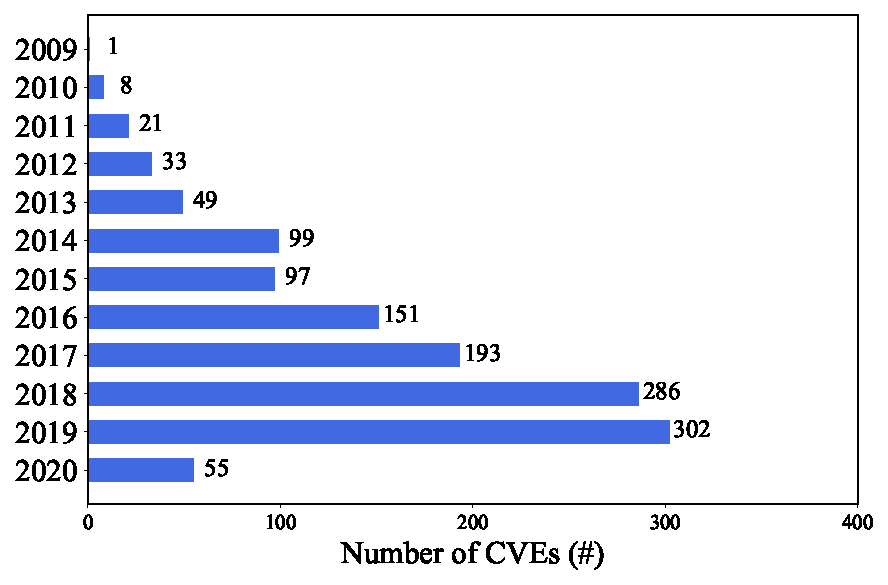
\includegraphics[scale=0.82]{fig/rq0-year.pdf}
    %\vspace{-5pt}
    \caption{数据集中漏洞年份统计}\label{fig:rq0-year}
    \centering
    \includegraphics[scale=0.82]{fig/rq0-language.pdf}
    \caption{数据集中漏洞程序语言分布统计}\label{fig:rq0-language}
\end{figure*}

% \begin{figure*}[t]
    
% \end{figure*}

本文还进一步分析了该深度数据集中\tocheck{1,295}个开源软件漏洞的年份和程序语言分布情况,以评估该数据集是否具有代表性。如图\ref{fig:rq0-year}所示,漏洞的数量逐年增加,这与Snyk报告\footnote{https://snyk.io/wp-content/uploads/sooss\_report\_v2.pdf.}的结果一致。此外,本文通过分析补丁中更改的源文件类型来确定漏洞的程序语言。如图\ref{fig:rq0-language}所示,深度数据集中的漏洞涵盖了七种较为常用的程序语言,具有较好的语言多样性。因此,可以认为该深度数据集对于开源软件漏洞数据库具有较好的代表性。


\section{RQ1:补丁覆盖率分析}\label{sec:coverage}
RQ1---补丁覆盖率分析,旨在评估漏洞数据库中开源软件漏洞的补丁缺失情况。对于包含10,070个开源软件漏洞的广度数据集,仅有\tocheck{4,602}个漏洞含有补丁,补丁覆盖率为45.7\%。本文还进一步分析了数据库$DB_A$和$DB_B$的补丁覆盖率。
如图\ref{fig:rq1-cves}所示,数据库$DB_A$和$DB_B$中共同拥有\tocheck{4,418}个漏洞,同时$DB_A$包含\tocheck{4,212}个特有的漏洞,$DB_B$包含\tocheck{1,440}个特有的漏洞。如图\ref{fig:rq1-cves-with-patches}所示,$DB_A$中,\tocheck{3,607(41.8\%)}的漏洞含有补丁;$DB_B$中,\tocheck{2,412(41.2\%)}的漏洞含有补丁。$DB_A$和$DB_B$数据库共有的\tocheck{4,418}个开源软件漏洞中,仅有\tocheck{1,417(32.0\%)}的漏洞含有补丁。$DB_A$和$DB_B$数据库一共有\tocheck{10,070}个开源软件漏洞(即广度数据集),而其中仅有\tocheck{4,602(45.7\%)}的漏洞含有补丁。
\begin{figure}[!t]
    \centering
    \begin{subfigure}[b]{0.45\textwidth}
    \centering
    \includegraphics[scale=0.98]{fig/rq1-CVE-IDs-VS.pdf}
    %\vspace{-5pt}
    \caption{开源软件漏洞}\label{fig:rq1-cves}
    \end{subfigure}
    \begin{subfigure}[b]{0.45\textwidth}
    \centering
    \includegraphics[scale=0.98]{fig/rq1-CVE-IDs-Patches-VS.pdf}
    %\vspace{-5pt}
    \caption{含补丁知识的开源软件漏洞}\label{fig:rq1-cves-with-patches}
    \end{subfigure}
    %\vspace{-10pt}
    \caption{$DB_A$与$DB_B$漏洞数据交集}\label{fig:intersection}
\end{figure}

% \begin{figure}[h]
%     \centering
%     \includegraphics[scale=0.98]{fig/rq1-CVE-IDs-VS.pdf}
%     \caption{开源软件漏洞数据}\label{fig:rq1-cves}
% \end{figure}

% \begin{figure}[h]
%     \centering
%     \includegraphics[scale=0.98]{fig/rq1-CVE-IDs-Patches-VS.pdf}
%     \caption{补丁的开源软件漏洞数据}\label{fig:rq1-cves-with-patches}
% \end{figure}

由此可见,数据库$DB_A$和$DB_B$中开源软件漏洞的补丁覆盖率都比较低,仅为41.8\%和41.2\%,这说明开源软件漏洞补丁缺失情况较为普遍。%而且可以看出,不同的漏洞数据库对\congyingEdit{OSS}漏洞的覆盖范围不同。
同时,这也体现出自动化补丁识别方法的必要性,可用于填补数据库中缺失的补丁。


\section{RQ2:补丁一致性分析}\label{sec:consistency}

\begin{table}[!t]
    \centering
    \small
    \caption{$DB_A$与$DB_B$补丁一致性分析结果}\label{table:consistency}
    %\vspace{-10pt}
    \begin{tabular}{|*{1}{C{4.4em}}|*{1}{C{3.8em}}*{1}{C{5.0em}}*{1}{C{5.0em}}|*{1}{C{3.6em}}*{1}{C{4.8em}}*{1}{C{5.0em}}|}
    \noalign{\hrule height 1pt}
    \multirow{2}{*}{补丁一致} & \multicolumn{3}{c|}{存在性不一致} & \multicolumn{3}{c|}{内容不一致} \\\cline{2-4}\cline{5-7}
     & 总数 & 某一数据库中无漏洞 & 某一数据库中无补丁 & 总数 & 补丁为包含关系 & 补丁非包含关系 \\\noalign{\hrule height 1pt}
    % \multirow{2}{*}{Cons.} & \multicolumn{3}{c|}{Existence Inconsistency} & \multicolumn{3}{c|}{Content Inconsistency} \\\cline{2-4}\cline{5-7}
    % & Total & No CVE & No Patch & Total & Inclusion & Difference \\\noalign{\hrule height 1pt}
    907 (19.7\%) & 3,185 (69.2\%) & 1,392 (30.2\%) & 1,793 (39.0\%) & 510 (11.1\%) & 176 (3.8\%) & 334 (7.3\%)\\
    % $DB_{A}$ vs. $DB_{C}$ & 3,659 & 73 (2.0\%) & 3,540 (96.7\%) & 2,523 (69.0\%) & 1,017 (27.8\%) & 46 (1.3\%) & 15 (0.4\%) & 31 (0.8\%) \\
    % $DB_{B}$ vs. $DB_{C}$ & 2,490 & 75 (3.0\%) & 2,397 (96.3\%) & 1,687 (67.8\%) & 710 (28.5\%) & 18 (0.7\%) & 7 (0.3\%) & 11 (0.4\%)\\
    \noalign{\hrule height 1pt}
    \end{tabular}
\end{table}

RQ2---补丁一致性分析,旨在评估不同漏洞数据库间漏洞补丁的不一致情况。
为了分析两个数据库之间的补丁一致性情况,本节仅分析带有补丁的漏洞,即图\ref{fig:rq1-cves-with-patches}中的漏洞。考虑到漏洞补丁的个数可能不唯一(即可能为一组补丁集),所以仅当两个数据库针对同一漏洞提供的补丁集完全相同时,才判定为补丁一致。本节将补丁不一致分为,存在性不一致和内容不一致两种情况。存在性不一致是指,某一个数据库存在该漏洞的补丁,而另一个数据库却不存在该漏洞,或是存在该漏洞却不存在相关补丁。内容不一致是指,两个数据库都存在该漏洞的补丁,但它们的补丁集并不完全一致,可以是包含关系或非包含关系。以上两种情况,分别反映了出数据库$DB_A$和$DB_B$中开源软件漏洞补丁的不完整性及不一致性。

表\ref{table:consistency}为补丁一致性分析的结果。其中,第一列为在$DB_A$和$DB_B$中具有一致补丁集的漏洞数量,第二至四列为补丁存在性不一致的漏洞数量,最后三列为都存在补丁但补丁集内容不一致的漏洞数量。可以发现:

\begin{enumerate}
    \item [(1)]\tocheck{4,602}个漏洞中,只有\tocheck{907(19.7\%)}的漏洞在$DB_A$和$DB_B$中有一致的补丁。
    \item [(2)]超过三分之二(即\tocheck{3,185 69.2\%})的漏洞在数据库$DB_A$和$DB_B$中存在补丁不一致的情况。其中\tocheck{1,392(30.2\%)}的漏洞不在$DB_{A}$或$DB_{B}$中,\tocheck{1,793(39.0\%)}的漏洞都存在于$DB_{A}$和$DB_{B}$中但在另一数据库中无补丁。
    \item [(3)]\tocheck{510(11.1\%)}的漏洞补丁都存在于$DB_{A}$和$DB_{B}$中,但补丁集不一致。其中,\tocheck{176(3.8\%)}的漏洞,某一个数据库的补丁集包含另一个数据库的补丁集;\tocheck{334(7.3\%)}的漏洞,$DB_{A}$和$DB_{B}$中的补丁集即不相同也不包含。
\end{enumerate}

这些结果表明,$DB_A$和$DB_B$间存在较多的补丁不一致情况,这很可能是由补丁不准确所导致,进而表明数据库中补丁的准确性需要进一步评估。

\section{RQ3:补丁类型分析}\label{sec:type}
\begin{table}[!t]
    \centering
    \small
    \caption{补丁类型分析结果}\label{table:type}
    %\vspace{-10pt}
    % \begin{tabular}{|*{1}{C{4.4em}}|*{1}{C{3.6em}}*{1}{C{5.0em}}*{1}{C{5.0em}}|}
    \begin{tabular}{|c|ccc|}
    \noalign{\hrule height 1pt}
    补丁总数 & GitHub代码提交 & SVN代码提交 & 其他Git平台代码提交 \\\noalign{\hrule height 1pt}
    3,043 & 2,852(93.7\%) & 136(4.5\%) & 55(1.8\%)\\\noalign{\hrule height 1pt}
    漏洞总数 & 仅GitHub代码提交 & 仅SVN代码提交 & 仅其他Git平台代码提交 \\\noalign{\hrule height 1pt}
    1,295 & 1,202(92.8\%) & 4(0.3\%) & 30(2.3\%)\\
    \noalign{\hrule height 1pt}
    \end{tabular}
\end{table}

RQ3---补丁类型分析,旨在表征开源软件漏洞的补丁类型。在章节\tocheck{\ref{sec:preparation}}中,基于人工收集的深度数据集共包含\tocheck{1,295}个漏洞及\tocheck{3,043}个补丁。本小节将基于该数据集分析漏洞的补丁类型。如表\ref{table:type}所示,\tocheck{3,043}个补丁中,\tocheck{2,852(93.7\%)}的补丁都是GitHub代码提交,这可能是因为GitHub在开源软件中被广泛使用;另外\tocheck{136(4.5\%)}的补丁为SVN代码提交,仅有\tocheck{55(1.8\%)}的补丁为来自其他Git平台的代码提交。

此外,从漏洞的角度来看,\tocheck{1,295}个漏洞中\tocheck{1,202(92.8\%)}的漏洞仅有GitHub提交类型的补丁,\tocheck{4(0.3\%)}的漏洞仅有SVN 提交类型的补丁。只有\tocheck{30(2.3\%)}的漏洞,补丁仅为来自其他Git平台的代码提交。由于很多项目是从SVN切换为Git管理,\tocheck{48(3.7\%)}的漏洞既有GitHub又有SVN提交类型的补丁。另外的\tocheck{11(0.8\%)}的漏洞,补丁为GitHub和其他Git平台的代码提交。

以上结果表明,开源软件漏洞的补丁类型主要为GitHub的代码提交(占比93.7\%),少部分为SVN代码提交,而极小部分为其他Git平台的代码提交。

\section{RQ4:补丁映射分析}\label{sec:cardinality}
\begin{figure}[h]
\centering
\includegraphics[scale=0.8]{fig/rq4-cardinality.pdf}
\vspace{-10pt}
\caption{漏洞及其补丁映射类型统计}\label{fig:rq4-cardinality}
\end{figure}

RQ4---补丁映射分析,旨在表征开源漏洞及其补丁之间的映射关系。基于深度数据集中\tocheck{1,295}个漏洞及其补丁,本节将分析开源漏洞及其补丁间在数量上的映射关系。本文将漏洞与其补丁之间的映射关系分为三种类型:一对一、\tocheck{一对一组}及一对多。

\textbf{一对一,}是指一个漏洞与其补丁在数量上为一对一的关系,即一个漏洞只需一个补丁即可修复,后文中简记为:\textit{SP}(Single Patch)。如图\ref{fig:rq4-cardinality}所示,深度数据集中\tocheck{567(43.8\%)}的漏洞与其补丁都是一对一的映射关系(\textit{SP})。

\textbf{一对一组,}是指一个漏洞有多个补丁,漏洞与其补丁在数量上非一对一关系。然而,这些补丁又都是等效的,任何一个补丁都足以修复该漏洞,后文中简记为:\textit{MEP}(Multiple Equivalent Patch)。等效补丁,是指代码变更完全一样的两个补丁提交,其主要有两种类型:
\begin{enumerate}
    \item [(1)] \textbf{请求提交(Requested Commit)VS. 合并提交(Merged Commits),}是指通过GitHub中的抓取(Pull Request)功能提交修复漏洞的代码更改。此时,请求提交和合并提交是该漏洞的等效补丁。例如,python-jose@89b463\footnote{https://github.com/mpdavis/python-jose/commit/89b46353b9f611e9da38de3d2fedf52331167b93}是请求提交,python-jose@73007d\footnote{https://github.com/mpdavis/python-jose/commit/73007d6887a7517ac07c6e755e494baee49ef513}是用于修复CVE-2016-7036的合并提交,这两个提交的代码变更完全相同,完全等效。
    \item [(2)] \textbf{SVN中代码提交 VS. GitHub中代码提交,}一些开源软件的仓库是后期由SVN迁移到GitHub的,因此,同一软件的SVN和GitHub的代码仓库中都有用于修补该漏洞的代码提交,且这两处提交的代码变更是完全一样且完全等效的。例如,软件james-hupa代码仓库从SVN迁移到了GitHub,SVN代码提交james-hupa@1373762\footnote{https://svn.apache.org/viewvc?view=revision\&revision=1373762}与GitHub 代码提交james-hupa@aff28a\footnote{https://github.com/apache/james-hupa/commit/aff28a8117a49969b0fc8cc9926c19fa90146d8d}是等效的。
\end{enumerate}

如图\ref{fig:rq4-cardinality}所示,深度数据集中\tocheck{195(15.1\%)}的漏洞与其补丁为一对一组映射关系(\textit{MEP})。

\textbf{一对多,}是指一个漏洞与其补丁在数量上为一对多的关系,即一个漏洞需多个非等效的补丁来修复。如图\ref{fig:rq4-cardinality}所示,深度数据集中\tocheck{533(41.2\%)}的漏洞与其补丁为一对多的映射关系,其可以再分为三种类型: 

\begin{enumerate}
\item [(1)] \textbf{多补丁,}一个漏洞需通过一个分支中的多个代码提交来修复。这是因为该漏洞较难修复需多次提交,或是后期发现初始的补丁提交不足以修复漏洞便追加了补丁提交。后文中将此简记为:\textit{MP}(Multiple Patch),占比\tocheck{7.8\%(101个漏洞)}。例如,CVE-2017-17837由三个独立的提交deltaspike@4e2502\footnote{https://github.com/apache/deltaspike/commit/4e2502358526b944fc5514c206d306e97ff271bb}、deltaspike@72e607\footnote{https://github.com/apache/deltaspike/commit/72e607f3be66c30c72b32c24b44e9deaa8e54608}和deltaspike@d95abe\footnote{https://github.com/apache/deltaspike/commit/d95abe8c01d256da2ce0a5a88f4593138156a4e5}修复。
\item [(2)] \textbf{多分支,}一个漏洞由多个分支中的多个补丁集修复。这是因为该漏洞影响了开源软件的多个版本,而每个版本又都在独立的分支上维护。后文中将此简记为:\textit{MB}(Multiple Branches),占比\tocheck{28.7\%(372个漏洞)}。例如,CVE-2019-19118影响了软件框架django的2.1.x、2.2.x、3.0.x和3.2.x版本,每个版本又都在独立的分支上维护。分布在四个分支的提交django@103ebe\footnote{https://github.com/django/django/commit/103ebe2b5ff1b2614b85a52c239f471904d26244}、django@36f580\footnote{https://github.com/django/django/commit/36f580a17f0b3cb087deadf3b65eea024f479c21}、django@092cd6\footnote{https://github.com/django/django/commit/092cd66cf3c3e175acce698d6ca2012068d878fa}和django@11c5e0\footnote{https://github.com/django/django/commit/11c5e0609bcc0db93809de2a08e0dc3d70b393e4}分别修复了受影响的四个版本。其中,django@103ebe与其他提交中的代码变更并不相同。
\item [(3)] \textbf{多仓库,}一个漏洞由多个代码仓库中的多个补丁集修复。这是因为该漏洞影响了多个开源软件或一个开源库的多个版本,而这些版本是分布在独立的代码仓库中维护的,所以会有来自不同仓库的提交。后文中将此简记为:\textit{MR}(Multiple Repositories),占比\tocheck{ 4.6\%(60个漏洞)}。例如,CVE-2016-5104影响了libimobiledevice和libusbmuxd两个开源软件,提交libimobiledevice@df1f5c\footnote{https://github.com/libimobiledevice/libimobiledevice/commit/df1f5c4d70d0c19ad40072f5246ca457e7f9849e}和libusbmuxd@4397b3\footnote{https://github.com/libimobiledevice/libusbmuxd/commit/4397b3376dc4e4cb1c991d0aed61ce6482614196}分修复了受影响的两个开源库。

\end{enumerate}
 %43.8 15.1\% 41.1
这些结果体现了开源软件漏洞与其补丁之间映射关系的多样性,超过\tocheck{40\%}的漏洞与其补丁具有一对多的映射关系。在后文设计自动化补丁识别方法时,应充分考虑该特征。

\section{RQ5:补丁准确性分析}\label{sec:accuracy}
\begin{table}[!t]
    \centering
    \small
    \caption{$DB_A$和$DB_B$补丁准确性评估结果}\label{table:accuracy}
    %\vspace{-10pt} 
    % \begin{tabular}{|*{1}{C{4.6em}}|*{1}{C{3.4em}}|*{3}{C{2.0em}}|*{3}{C{2.0em}}|}
    \begin{tabular}{|c|c|ccc|ccc|}
    \noalign{\hrule height 1pt}
    \multirow{2}{*}{映射类型} & \multirow{2}{*}{数量} &  \multicolumn{3}{c|}{$DB_A$} & \multicolumn{3}{c|}{$DB_B$} \\\cline{3-8}
    & & Pre. & Rec. & F1 & Pre. & Rec. & F1 \\
    \noalign{\hrule height 1pt}
    1:1 (SP) & 567       & 0.908 & 0.915 & 0.910   & 0.900 & 0.921 & 0.906   \\
    1:$i$ (MEP) & 195    & 0.935 & 0.898 & 0.902  & 0.924 & 0.909  & 0.906   \\
    1:$n$ (MP) & 101     & 0.923 & 0.483 & 0.616  & 0.911 & 0.520 & 0.638    \\
    1:$n$ (MB) & 372     & 0.941 & 0.510 & 0.620  & 0.932 & 0.436 & 0.555    \\
    1:$n$ (MR) & 60      & 0.913 & 0.610 & 0.695  & 0.964 & 0.526 & 0.636   \\\hline
    总计 & 1,295       & 0.923 & 0.748 & 0.793  & 0.917 & 0.730 & 0.771     \\
    \noalign{\hrule height 1pt}
    \end{tabular}
\end{table}

RQ5---补丁准确性分析,旨在评估不同漏洞数据库中漏洞补丁的准确性。
本文使用精确率(precision)、召回率(recall)和F1值(F1-score)作为评估补丁准确性的指标。对于具有等效补丁的漏洞,则进行特殊计算。例如,对于具有两个等效补丁的漏洞,若数据库提供两个等效补丁中的任意一个,精确率和召回率都为1;若数据库提供两个等效补丁中的一个补丁和另一个不相关的补丁,那么精确率为0.5,召回率为1。其他情况,依此类推。

表\ref{table:accuracy}为$DB_A$和$DB_B$的补丁准确性评估结果。其中,第一列为漏洞与补丁的映射类型,第二列为该映射类型的漏洞数量,最后六列分别为数据库$DB_A$和$DB_B$中漏洞补丁的准确率、召回率和F1值。结果表明,对于\textit{SP}和\textit{MEP}类型的漏洞,$DB_A$和$DB_B$可达到约90\%的精确率和召回率;对于\textit{MP}、\textit{MB}和\textit{MR}类型的漏洞,$DB_A$和$DB_B$可达到90\%以上的高精确率,但仅有约50\%的召回率。例如,对于漏洞CVE-2017-17837,$DB_A$和$DB_B$仅报告三个补丁中的一个;对于漏洞CVE-2019-19118,$DB_A$报告了四个补丁中的两个,而$DB_B$仅报告四个补丁中的一个。

这说明漏洞数据库$DB_A$和$DB_B$具有较高的精确率,但经常会遗漏一些漏洞的补丁,尤其是对于具有多个补丁的漏洞。对于漏洞数据库用户来说,这会给漏洞的及时检测和修复带来较大困难。%,这也反映出自动化补丁识别方法的必要性。

\section{研究发现}
本文针对开源软件漏洞补丁的经验研究,共涉及五个研究问题。其中,RQ1补丁覆盖率分析、RQ2补丁一致性分析和RQ5补丁准确性分析的结果旨在从不同的角度评估补丁质量,并挖掘出对自动化补丁识别方法的需求。RQ3补丁类型分析和RQ4补丁准确性分析旨在从不同角度捕捉开源软件漏洞补丁的特征,并为自动化补丁识别方法的设计提供启发。该经验研究中,本文主要有以下发现:

\begin{enumerate}
    \item [(1)]商业漏洞数据库中开源软件漏洞补丁的质量并不理想,体现在:(i)开源软件漏洞补丁缺失情况较为普遍,商业数据库$DB_A$和$DB_B$中开源软件漏洞的补丁覆盖率仅为41.8\%和41.2\%。(ii)商业漏洞数据库$DB_A$和$DB_B$具有较高的精确率,但经常会遗漏一些漏洞的补丁,尤其是对于具有多个补丁的漏洞。对于安全服务用户来说,这会给漏洞的及时检测和修复带来较大困难。这体现出当前开源软件漏洞数据库的不足,以及利用自动化补丁识别方法完善漏洞数据的需求。
    \item [(2)]开源软件漏洞补丁在类型、映射关系方面有一定的特殊性,设计自动化补丁识别方法时应充分考虑。体现在:(i)93.7\%的补丁都为GitHub代码提交的形式。(ii)开源软件漏洞与其补丁之间映射关系具有多样性,超过40\%的漏洞与其补丁具有一对多的映射关系。
\end{enumerate}

